\begin{remark*}[Exposition]
Before metric topology begins, the metric already supplies quantitative
measurements.  This section records the set-geometry notions currently
formalized in Lean: diameter, the set of point-to-set distances, and basic
order facts about those constructions.
\end{remark*}

\begin{definitionbox}{Definition --- Diameter Distance Set}
\begin{definition}[Diameter Distance Set]\label{def:metric-diameter-distance-set}
Let \((X,d)\) be a metric space and let \(A\subseteq X\).  The
\emph{diameter distance set} of \(A\) is
\[
  D(A)
  :=
  \{\,r\in\mathbb{R}:\exists a,b\in A\text{ such that }r=d(a,b)\,\}.
\]
\end{definition}
\end{definitionbox}

\begin{remark*}[Standard quantified statement]
\[
r\in D(A)
\quad\Longleftrightarrow\quad
\exists a\in A\,\exists b\in A{:}\ r=d(a,b).
\]
\end{remark*}

\begin{remark*}[Predicate reading]
\[
D(A)=\{\,d(a,b):a,b\in A\,\}
\]
means that the set \(D(A)\) is built from all metric distances witnessed by
pairs of points in \(A\).
\end{remark*}

\begin{remark*}[Interpretation]
The diameter distance set collects the pairwise distances that actually occur
between points of \(A\).  It is the raw set whose supremum becomes the
diameter.
\end{remark*}

\LeanFormalizes{def:metric-diameter-distance-set}{lra-lean}{LRA.VolumeIV.MetricSpaces.SetGeometry.Diameter}{diameterSet}{statement}

\begin{dependencies}
\begin{itemize}
  \item \hyperref[def:metric-space]{Definition: Metric Space}
\end{itemize}
\end{dependencies}

\begin{definitionbox}{Definition --- Diameter}
\begin{definition}[Diameter]\label{def:metric-diameter}
Let \((X,d)\) be a metric space and let \(A\subseteq X\).  The
\emph{diameter} of \(A\) is
\[
  \operatorname{diam}(A)
  :=
  \sup D(A).
\]
\end{definition}
\end{definitionbox}

\begin{remark*}[Standard quantified statement]
\[
\operatorname{diam}(A)
=
\sup\{\,d(a,b):a,b\in A\,\}.
\]
\end{remark*}

\begin{remark*}[Interpretation]
The diameter records the largest distance needed to travel between two points
of \(A\).  It measures internal spread rather than location.
\end{remark*}

\begin{figure}[htbp]
\centering
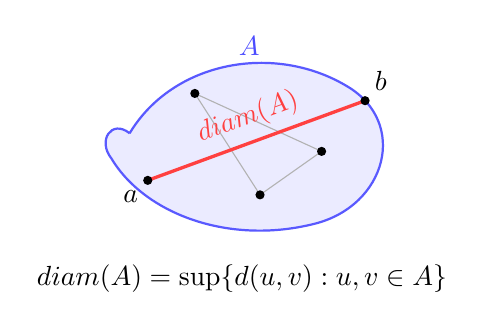
\begin{tikzpicture}[scale=0.92,>=stealth]
  \fill[blue!8]
    (0.0,0.0) .. controls (0.6,1.0) and (2.0,1.25) .. (3.0,0.65)
    .. controls (3.85,0.15) and (3.55,-1.0) .. (2.55,-1.25)
    .. controls (1.35,-1.55) and (0.2,-1.1) .. (-0.25,-0.35)
    .. controls (-0.45,-0.1) and (-0.25,0.2) .. (0.0,0.0);
  \draw[blue!65,thick]
    (0.0,0.0) .. controls (0.6,1.0) and (2.0,1.25) .. (3.0,0.65)
    .. controls (3.85,0.15) and (3.55,-1.0) .. (2.55,-1.25)
    .. controls (1.35,-1.55) and (0.2,-1.1) .. (-0.25,-0.35)
    .. controls (-0.45,-0.1) and (-0.25,0.2) .. (0.0,0.0);

  \coordinate (a) at (0.25,-0.65);
  \coordinate (b) at (3.25,0.45);
  \coordinate (c) at (0.9,0.55);
  \coordinate (d) at (1.8,-0.85);
  \coordinate (e) at (2.65,-0.25);

  \draw[gray!60] (c) -- (e);
  \draw[gray!60] (c) -- (d);
  \draw[gray!60] (d) -- (e);
  \draw[red!75,very thick] (a) -- (b)
    node[midway,above,sloped] {\(\operatorname{diam}(A)\)};

  \foreach \p/\lab/\pos in {a/a/below left,b/b/above right,c/{}/above,d/{}/below,e/{}/right}
  {
    \fill[black] (\p) circle (1.8pt);
    \node[\pos] at (\p) {\(\lab\)};
  }

  \node[blue!70] at (1.65,1.2) {\(A\)};
  \node[align=center] at (1.55,-2.0)
    {\(\operatorname{diam}(A)=\sup\{d(u,v):u,v\in A\}\)};
\end{tikzpicture}

\caption{The diameter of \(A\) is the supremum of the pairwise distances
between points of \(A\).}
\label{fig:metric-diameter-distance-set}
\end{figure}

\LeanFormalizes{def:metric-diameter}{lra-lean}{LRA.VolumeIV.MetricSpaces.SetGeometry.Diameter}{diameter}{statement}

\begin{dependencies}
\begin{itemize}
  \item \hyperref[def:metric-diameter-distance-set]{Definition: Diameter Distance Set}
\end{itemize}
\end{dependencies}

\begin{theorembox}{Theorem}
\begin{theorem}[Diameter Distance Sets are Monotone]
\label{thm:metric-diameter-set-monotone}
Let \((X,d)\) be a metric space and let \(A,B\subseteq X\).  If
\(A\subseteq B\), then
\[
  D(A)\subseteq D(B).
\]
\hyperref[prf:metric-diameter-set-monotone]{\textit{Go to proof.}}
\end{theorem}
\end{theorembox}

\begin{remark*}[Standard quantified statement]
\[
A\subseteq B
\Longrightarrow
D(A)\subseteq D(B).
\]
\end{remark*}

\begin{remark*}[Interpretation]
Every pair of points from \(A\) is also a pair of points from \(B\), so every
distance witnessed inside \(A\) is witnessed inside \(B\).
\end{remark*}

\LeanFormalizes{thm:metric-diameter-set-monotone}{lra-lean}{LRA.VolumeIV.MetricSpaces.SetGeometry.Diameter}{diameterSet_mono}{checked}

\begin{dependencies}
\begin{itemize}
  \item \hyperref[def:metric-diameter-distance-set]{Definition: Diameter Distance Set}
\end{itemize}
\end{dependencies}

\begin{theorembox}{Theorem}
\begin{theorem}[Diameter is Monotone Under Inclusion]
\label{thm:metric-diameter-monotone-under-inclusion}
Let \((X,d)\) be a metric space and let \(A,B\subseteq X\).  If
\(A\subseteq B\), \(D(A)\) is nonempty, and \(D(B)\) is bounded above, then
\[
  \operatorname{diam}(A)\leq \operatorname{diam}(B).
\]
\hyperref[prf:metric-diameter-monotone-under-inclusion]{\textit{Go to proof.}}
\end{theorem}
\end{theorembox}

\begin{remark*}[Standard quantified statement]
\[
A\subseteq B,\quad D(A)\neq\varnothing,\quad D(B)\text{ bounded above}
\Longrightarrow
\operatorname{diam}(A)\leq \operatorname{diam}(B).
\]
\end{remark*}

\begin{remark*}[Interpretation]
Passing to a larger set can only add candidate pairwise distances.  When the
relevant suprema are controlled, the diameter cannot decrease by enlarging
the set.
\end{remark*}

\LeanFormalizes{thm:metric-diameter-monotone-under-inclusion}{lra-lean}{LRA.VolumeIV.MetricSpaces.SetGeometry.Diameter}{diameter_monotone_under_inclusion}{checked}

\begin{dependencies}
\begin{itemize}
  \item \hyperref[def:metric-diameter]{Definition: Diameter}
  \item \hyperref[thm:metric-diameter-set-monotone]{Theorem: Diameter Distance Sets are Monotone}
\end{itemize}
\end{dependencies}

\begin{definitionbox}{Definition --- Point-to-Set Distance Set}
\begin{definition}[Point-to-Set Distance Set]\label{def:metric-point-set-distance-set}
Let \((X,d)\) be a metric space, let \(x\in X\), and let \(A\subseteq X\).
The \emph{point-to-set distance set} from \(x\) to \(A\) is
\[
  D(x,A)
  :=
  \{\,d(x,a):a\in A\,\}.
\]
\end{definition}
\end{definitionbox}

\begin{remark*}[Standard quantified statement]
\[
r\in D(x,A)
\quad\Longleftrightarrow\quad
\exists a\in A{:}\ r=d(x,a).
\]
\end{remark*}

\begin{remark*}[Interpretation]
The point-to-set distance set records all distances from the fixed point
\(x\) to points of \(A\).
\end{remark*}

\LeanFormalizes{def:metric-point-set-distance-set}{lra-lean}{LRA.VolumeIV.MetricSpaces.SetGeometry.DistanceToSet}{distanceSet}{statement}

\begin{dependencies}
\begin{itemize}
  \item \hyperref[def:metric-space]{Definition: Metric Space}
\end{itemize}
\end{dependencies}

\begin{definitionbox}{Definition --- Distance from a Point to a Set}
\begin{definition}[Distance from a Point to a Set]\label{def:metric-point-set-distance}
Let \((X,d)\) be a metric space, let \(x\in X\), and let \(A\subseteq X\).
The \emph{distance from \(x\) to \(A\)} is
\[
  d(x,A):=\inf D(x,A).
\]
\end{definition}
\end{definitionbox}

\begin{remark*}[Standard quantified statement]
\[
d(x,A)=\inf\{\,d(x,a):a\in A\,\}.
\]
\end{remark*}

\begin{remark*}[Interpretation]
The number \(d(x,A)\) measures how close \(x\) can get to \(A\).  The
infimum may be achieved by a point of \(A\), but it need not be achieved in
every metric space.
\end{remark*}

\begin{figure}[htbp]
\centering
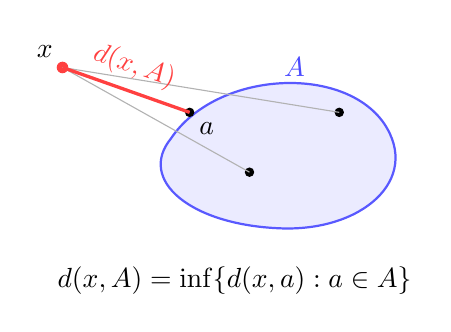
\begin{tikzpicture}[scale=0.95,>=stealth]
  \fill[blue!8]
    (0.0,0.0) .. controls (0.6,0.9) and (2.3,1.0) .. (2.85,0.2)
    .. controls (3.35,-0.55) and (2.55,-1.25) .. (1.45,-1.2)
    .. controls (0.25,-1.15) and (-0.45,-0.55) .. (0.0,0.0);
  \draw[blue!65,thick]
    (0.0,0.0) .. controls (0.6,0.9) and (2.3,1.0) .. (2.85,0.2)
    .. controls (3.35,-0.55) and (2.55,-1.25) .. (1.45,-1.2)
    .. controls (0.25,-1.15) and (-0.45,-0.55) .. (0.0,0.0);

  \coordinate (x) at (-1.45,0.95);
  \coordinate (a) at (0.25,0.35);
  \coordinate (b) at (1.05,-0.45);
  \coordinate (c) at (2.25,0.35);
  \coordinate (p) at (0.25,0.35);

  \foreach \q in {a,b,c}
    \fill[black] (\q) circle (1.8pt);

  \fill[red!75] (x) circle (2.2pt);
  \node[above left] at (x) {\(x\)};
  \node[blue!70] at (1.65,0.95) {\(A\)};

  \draw[gray!60] (x) -- (b);
  \draw[gray!60] (x) -- (c);
  \draw[red!75,very thick] (x) -- (p)
    node[midway,above,sloped] {\(d(x,A)\)};

  \node[below right] at (p) {\(a\)};
  \node[align=center] at (0.85,-1.9)
    {\(d(x,A)=\inf\{d(x,a):a\in A\}\)};
\end{tikzpicture}

\caption{The point-to-set distance \(d(x,A)\) is the infimum of the distances
from \(x\) to points of \(A\).}
\label{fig:metric-point-set-distance}
\end{figure}

\LeanFormalizes{def:metric-point-set-distance}{lra-lean}{LRA.VolumeIV.MetricSpaces.SetGeometry.DistanceToSet}{distanceToSet}{statement}

\begin{dependencies}
\begin{itemize}
  \item \hyperref[def:metric-point-set-distance-set]{Definition: Point-to-Set Distance Set}
\end{itemize}
\end{dependencies}

\begin{theorembox}{Theorem}
\begin{theorem}[Point-to-Set Distance Sets are Bounded Below]
\label{thm:metric-distance-set-bounded-below}
Let \((X,d)\) be a metric space, let \(x\in X\), and let \(A\subseteq X\).
Then \(D(x,A)\) is bounded below by \(0\).
\hyperref[prf:metric-distance-set-bounded-below]{\textit{Go to proof.}}
\end{theorem}
\end{theorembox}

\begin{remark*}[Standard quantified statement]
\[
\forall r\in D(x,A){:}\quad 0\leq r.
\]
\end{remark*}

\begin{remark*}[Interpretation]
Every element of \(D(x,A)\) is a metric distance, and metric distances are
nonnegative.
\end{remark*}

\LeanFormalizes{thm:metric-distance-set-bounded-below}{lra-lean}{LRA.VolumeIV.MetricSpaces.SetGeometry.DistanceToSet}{distanceSet_bddBelow}{checked}

\begin{dependencies}
\begin{itemize}
  \item \hyperref[def:metric-point-set-distance-set]{Definition: Point-to-Set Distance Set}
  \item \hyperref[def:metric-on-set]{Definition: Metric}
\end{itemize}
\end{dependencies}

\begin{theorembox}{Theorem}
\begin{theorem}[Point-to-Set Distance is Bounded by Witness Distances]
\label{thm:metric-distance-to-set-le-distance-to-point-of-mem}
Let \((X,d)\) be a metric space, let \(x\in X\), let \(A\subseteq X\), and let
\(a\in A\).  Then
\[
  d(x,A)\leq d(x,a).
\]
\hyperref[prf:metric-distance-to-set-le-distance-to-point-of-mem]{\textit{Go to proof.}}
\end{theorem}
\end{theorembox}

\begin{remark*}[Standard quantified statement]
\[
a\in A
\Longrightarrow
d(x,A)\leq d(x,a).
\]
\end{remark*}

\begin{remark*}[Interpretation]
The infimum of all distances from \(x\) to \(A\) is no larger than any one
particular witnessed distance from \(x\) to a point of \(A\).
\end{remark*}

\LeanFormalizes{thm:metric-distance-to-set-le-distance-to-point-of-mem}{lra-lean}{LRA.VolumeIV.MetricSpaces.SetGeometry.DistanceToSet}{distanceToSet_le_distance_to_point_of_mem}{checked}

\begin{dependencies}
\begin{itemize}
  \item \hyperref[def:metric-point-set-distance]{Definition: Distance from a Point to a Set}
\end{itemize}
\end{dependencies}

\begin{theorembox}{Theorem}
\begin{theorem}[Point-to-Set Distance is Zero at Points of the Set]
\label{thm:metric-distance-to-set-zero-of-mem}
Let \((X,d)\) be a metric space, let \(A\subseteq X\), and let \(x\in A\).
Then
\[
  d(x,A)=0.
\]
\hyperref[prf:metric-distance-to-set-zero-of-mem]{\textit{Go to proof.}}
\end{theorem}
\end{theorembox}

\begin{remark*}[Standard quantified statement]
\[
x\in A
\Longrightarrow
d(x,A)=0.
\]
\end{remark*}

\begin{remark*}[Interpretation]
If \(x\) is already in \(A\), then one candidate distance in \(D(x,A)\) is
\(d(x,x)=0\).  Nonnegativity prevents the infimum from being smaller.
\end{remark*}

\LeanFormalizes{thm:metric-distance-to-set-zero-of-mem}{lra-lean}{LRA.VolumeIV.MetricSpaces.SetGeometry.DistanceToSet}{distanceToSet_eq_zero_of_mem}{checked}

\begin{dependencies}
\begin{itemize}
  \item \hyperref[def:metric-point-set-distance]{Definition: Distance from a Point to a Set}
  \item \hyperref[thm:metric-distance-set-bounded-below]{Theorem: Point-to-Set Distance Sets are Bounded Below}
  \item \hyperref[thm:metric-distance-to-set-le-distance-to-point-of-mem]{Theorem: Point-to-Set Distance is Bounded by Witness Distances}
\end{itemize}
\end{dependencies}
